\section{When the scheduling recommendation changes}
\label{sec:scheduling-results}
Vector size alone does not determine the useful schedule. Table~\ref{tab:scheduling-sensitivity} compares each order with original order under the same request boundaries and memory settings. Figure~\ref{fig:scheduling-sensitivity} shows the individual split effects as well as paired intervals. These are six separate interventions around the default, not a full interaction study of every possible combination.

\begin{table}[htbp]\centering\small
\caption[Scheduling sensitivity: paired comparisons]{Cycle differences (\%) from matching original-order BFS replay: mean and paired 95\% interval over ten reference splits. Negative means fewer service cycles. Only the named setting changes from the default; 128 bytes is a hypothetical footprint.}\label{tab:scheduling-sensitivity}
\resizebox{\textwidth}{!}{\begin{tabular}{lrrr}
\toprule
Condition & Bytes & Sorted & Round-robin \\
\midrule
Default (64 outstanding) & 512 & +0.19 [+0.13, +0.24] & -14.58 [-14.64, -14.51] \\
Default (64 outstanding) & 128 & +0.17 [+0.12, +0.21] & +3.43 [+3.31, +3.55] \\
16 outstanding & 512 & +0.28 [+0.25, +0.31] & -33.08 [-33.21, -32.94] \\
16 outstanding & 128 & +0.71 [+0.67, +0.74] & -10.61 [-10.68, -10.54] \\
32 outstanding & 512 & +0.26 [+0.22, +0.31] & -21.86 [-21.95, -21.78] \\
32 outstanding & 128 & +0.29 [+0.23, +0.35] & +1.62 [+1.52, +1.73] \\
128 outstanding & 512 & +0.19 [+0.13, +0.24] & -14.58 [-14.64, -14.51] \\
128 outstanding & 128 & +0.17 [+0.12, +0.21] & +3.43 [+3.31, +3.55] \\
Candidate batches of 2 & 512 & -0.07 [-0.09, -0.06] & -7.77 [-7.79, -7.76] \\
Candidate batches of 2 & 128 & -0.08 [-0.11, -0.06] & -1.48 [-1.51, -1.46] \\
Candidate batches of 8 & 512 & +0.13 [+0.07, +0.18] & -15.55 [-15.60, -15.50] \\
Candidate batches of 8 & 128 & +0.13 [+0.08, +0.17] & -2.48 [-2.52, -2.43] \\
Alternative address mapping & 512 & +3.52 [+3.34, +3.70] & +112.71 [+111.01, +114.41] \\
Alternative address mapping & 128 & -0.34 [-0.36, -0.33] & +42.59 [+41.98, +43.19] \\
\bottomrule
\end{tabular}
}
\end{table}

At 16 outstanding transactions, round-robin changes the 128-byte result to \SchedInflightSixteenRRCompact\%, compared with \SchedDefaultRRCompact\% at the default limit of 64. The same representation can therefore benefit from interleaving when less work fits inside the request bound. At 512 bytes, the 16-outstanding result is \SchedInflightSixteenRRFloat\%. This is evidence about the exposed work under these limits, rather than a universal byte-size threshold.

The alternative address mapper is a stronger counterexample to an unconditional round-robin rule: its differences are \SchedAlternateMappingRRFloat\% and \SchedAlternateMappingRRCompact\% at 512 and 128 bytes. Physical address decoding changes which chunks share banks and rows. Sorting also needs a conditional interpretation: under this mapper its 128-byte difference is \SchedAlternateMappingSortCompact\%, whereas it is slower at the default. Sorting also gives small reductions with two-vector batches: \SchedBatchTwoSortFloat\% and \SchedBatchTwoSortCompact\% at the two widths. The appropriate conclusion is to test completed service under the target execution settings, rather than to reject or endorse an order from its name.

Candidate batches test a different constraint. Limiting a group to two or eight vectors adds completion boundaries and changes the alternatives' opportunity to overlap. The matching original-order denominator includes the same boundaries. These comparisons isolate the value of ordering \emph{within that batch model}; a percentage here cannot by itself rank batch sizes or predict a scratch-memory implementation.

Raising the outstanding limit from 64 to 128 reproduces the default total cycles in \SchedRaisedLimitEqual{} of the 60 matching split/footprint/order records. The largest observed default peak is \SchedDefaultPeak{} uncompleted reads. The default cap therefore leaves unused capacity in these records; increasing a nonbinding bound does not supply more useful work by itself. This observation does not isolate the read-buffer size as the sole limiting factor.

\begin{figure}[htbp]\centering
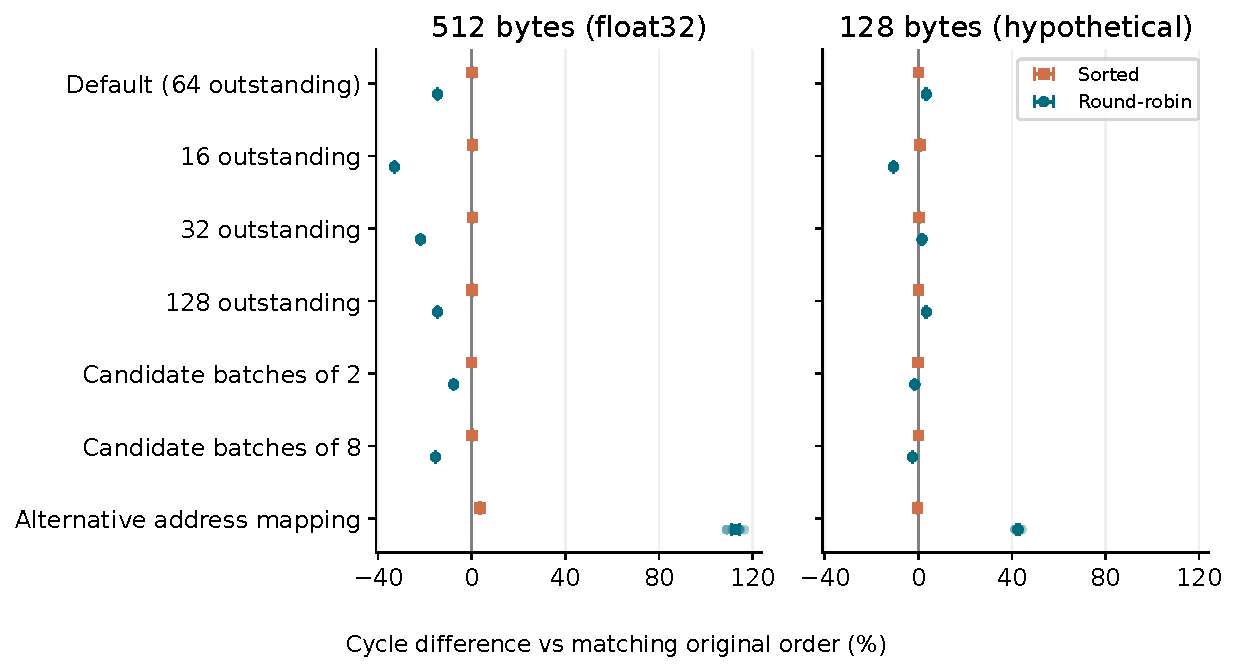
\includegraphics[width=\textwidth]{generated/scheduling_sensitivity.pdf}
\caption[How execution constraints change request ordering]{Scheduling differences against matching original-order BFS. Faint points are the ten split effects; larger markers and bars show their mean and paired 95\% interval. Both footprints use the same horizontal scale. The large alternative-mapper loss remains visible rather than being omitted to enlarge the default gain.}\label{fig:scheduling-sensitivity}
\end{figure}

Per-query savings, faster-query fractions and changes in the empirical 95th percentile are retained in Appendix~\ref{app:scheduling-detail}. They describe variation within each case and do not create additional independent repetitions. The result supports profiling a schedule for the execution configuration, which the next section evaluates with training queries.
